\section{Eggholder Function}
\label{sec:app:test:eggholder}
  The \emph{Eggholder function} is a widely-used non-convex function in the 
  field of optimization, particularly for benchmarking optimization algorithms.
  The function is notorious for its multitude of local minima, presenting a 
  complex search space that challenges the robustness and capability of an 
  optimization algorithm to locate the global minimum.

  \begin{definition}[Eggholder Function]
  Formally, the \emph{Eggholder Function} is represented as a mapping 
  \(\mathbb{R}^2 \to \mathbb{R}\), and is mathematically defined as:

  \begin{equation}
    f(x,\, y) = 
      -(y + 47) \sin\left(\sqrt{\left| \frac{x}{2} + (y + 47) \right|}\right) 
      - x \sin\left(\sqrt{\left| x - (y + 47) \right|}\right)
  \end{equation}

  where the typical domain for evaluation spans \(-512 \leq x, y \leq 512\).
  \end{definition}

  The Eggholder function's global minimum resides at \((512,\, 404.2319)\), 
  delivering a function value of \(f(x,\, y) = -959.6407\).

  Visual representations of the function can enhance understanding of its 
  complexity.
  Figure \vref{fig:app:test:eggholder} offers both contour and surface plots of 
  the Eggholder function.

  \begin{figure}[ht!]
    \centering
    \begin{subfigure}[b]{0.45\textwidth}
      \centering
      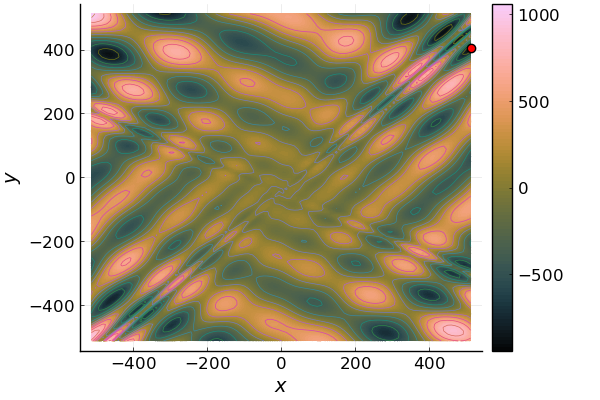
\includegraphics[width=\textwidth]
        {img/test_functions/eggholder_contour.png}
      \caption{
        A contour plot of the Eggholder function, displaying its intricate
        landscape.
        The red dot signifies the location of the global minimum.
      }
      \label{fig:app:test:eggholder:contour}
    \end{subfigure}
    \hfill
    \begin{subfigure}[b]{0.45\textwidth}
      \centering
      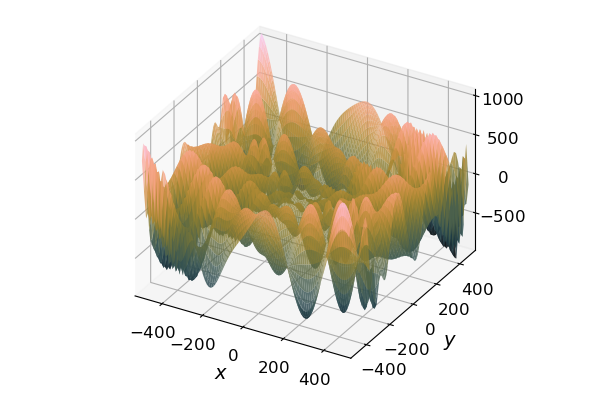
\includegraphics[width=\textwidth]
        {img/test_functions/eggholder_surface.png}
      \caption{
        A 3D surface plot of the Eggholder function, allowing a more 
        comprehensive visualization of its local and global minima.
      }
      \label{fig:app:test:eggholder:surface}
    \end{subfigure}
    \caption{
      Contour and surface visualizations of the Eggholder function, showcasing 
      its intricate topology
    }
    \label{fig:app:test:eggholder}
  \end{figure}
